\documentclass{./llncs2e/llncs}
\usepackage{graphicx}
%%%%
\usepackage{fixltx2e}
%%%%
\usepackage{mathtools}
%%%%
\usepackage[nolist,nohyperlinks]{acronym}
%%%%
\usepackage[section]{placeins}
%%%% Maintain images and tables within their respective sections
\usepackage{float}
%%%%
\usepackage[utf8]{inputenc}
%%%% Declare that we're using utf8 encoding
\usepackage{listings}
%%%% Include package for listings


% 
% Change the margins
% 
% \usepackage[margin=2.9cm]{geometry}

\begin{document}
\title{A Browser-based Interactive Development Environment for Generative Design}

\subtitle{Your Thesis subtitle}
\author{Pedro Alfaiate, pedro.alfaiate@tecnico.ulisboa.pt}
\institute{Instituto Superior Técnico}

\maketitle

%----------------------------------------------------
%NAVabstract
\begin{abstract}

\end{abstract}
%----------------------------------------------------
%NAVkeywords
\begin{keywords}

\end{keywords}
%----------------------------------------------------
%NAVintroduction
\section{Introduction (2/3pgs)}
	Programming is becoming an essential way of expressing ideas in a way a computer can understand them.

	Once a computer can understand an idea (or process) it can apply it as many times as we want.

	Expressing ideas/processes in a way a computer understands requires us to specify every detail of what we have in mind (sometimes too much) which forces us to really understand what it is.

	Many people have understood the power that comes from having a computer (or machine) doing lots of mechanical work and so have adopted programming as a new tool.

	Still, programming as it is normally present requires a lot of discipline on the part of the programmer to keep what he is expressing understandable.

	To ease the task of programming right, programming languages such as Logo\cite{papert1999logo}, Scratch\cite{Resnick:2009:SP:1592761.1592779} and Smalltalk\cite{goldberg1983smalltalk} have been developed. Such languages provide environments with strong metaphors that guide the programmer as he learns and uses it to create increasingly complex programs (or express complex ideas).

	Although the languages referred above provide great environments to think about what is being programmed, they are also often viewed as too restrictive and haven't spread enough to be considered useful (they are too restricted, seen has ``for children'', not useful and/or not known).

	These languages restrict themselves to pedagogic concepts and lack functionality that is needed for real world application.

	Whatever the reason for not being used, they have been replaced by other more well-known languages. Some of those languages are Lua, Python and Javascript \textbf{REFs?}. These three are all dynamic languages and were designed to be easy to understand and to use by people with little programming knowledge. They are dynamic (checked on runtime, change on runtime, ...), have loose syntax and have loose typing. They are ``more forgiving''.

	Being aimed at beginners doesn't mean that those languages require no amount of training to be used. The basic concepts of those languages still have to be understood. A way to understand those concepts is to attend a programming course. This is usually not an option for people that ``just want to try programming'' as they already have a busy schedule.

	Online courses are an alternative to ``in person'' courses. They don't require people to move to a school to attend classes and their classes are often recorded. They are much more flexible and thus attractive to those that want to try programming.

	Many online courses have appeared on the topic of programming. Many of them use the languages from above to teach programming. Coursera\footnote{https://www.coursera.org/} and Khanacademy\footnote{https://www.khanacademy.org/} are examples of sites that provide such courses. (opinion: these courses often try to appeal ``too much'' to their audience, focusing just on the results and end up not teaching the core of programming, understanding the problem).

	Most online programming courses of today don't even require their attendants to install anything on their computers. The only required software is a modern web browser. More so, the languages used by them include not only Javascript (with native support from the web browser) but also any dynamic language.

	The concept of not needing to install anything apart from a web browser is a general trend in today's software market(ing). From common desktop tools like Google Docs\footnote{https://docs.google.com/}, available from the browser even with cloud storage, to professional software development environments like Cloud9\footnote{https://c9.io/}. Everything is going to the browser.

	Following the trend of using programming in their work, architects started using programming to generate the 3D models of the buildings they ``come up with''. They use a process called Generative Design\cite{terzidis2003expressive}\cite{Maeda:2001:DN:559503}.

	Using Generative Design enables the designer to easily create variants of his design by changing a small set of parameters. Those parameters are used by the computer to run the algorithm, written by the designer, to generate an ``instance'' of his design. \cite{Santos20144} \textbf{Ref Sketchpad master drawings}

	There are several environments/software packages that enable people to use Generative Design to make 3D models. First, after recognizing the advantages it brings to its users\footnote{Many architecture and design projects require a lot of repetition, the \emph{forte} of programming/machines.}, all major CAD softwares used by architects support Generative Design through dedicated programming environments. There are also standalone programming environments like Processing\cite{reas2007processing} or Rosetta\cite{de2012modern}; the first is a programming environment for the visual (or other) arts and the second is an environment specifically for Generative Design that aims to separate the design from the CAD its results are ``displayed'' in. As pure programming environments, these last two don't consider/provide direct manipulation as a primary tool in their approach.

	Like online programming courses, programing environments for Generative Design can move to the web browser. Complementarily to not requiring installation, moving to the browser (or to a website) also makes programming environments available from anywhere a browser is found, be it a computer running Windows, Mac OS X or a Linux or even an Android tablet. They would require no installation, would be ubiquitous and would be OS independent; contrasting with major CADs, like AutoCAD\footnote{Currently AutoCAD has a full-featured version running on Windows and a less feature rich version running on Mac OS.}, that are tied to one OS or have serious drawbacks against using other OSs.

	There aren't any known Generative Design environments that run in the web browser. This is in part because until now the browser didn't have the necessary technology to support performant 3D applications. This is not the case right now. Clara.io\cite{Houston:2013:CFC:2503673.2503681}, an online 3D modeler (like 3ds Max) and \textbf{*insert js webapp here*} show that it is possible to build web browser based applications that are on pair with their desktop analogs.

	We propose a web browser based Generative Design environment. Such environment will allow architects, or anyone interested in Generative Design, to edit Generative Design programs and visualize their results while not requiring any installation. It will thus allow them to do Generative Design on any computer that has a modern browser. Not being tied to a workstation will allow them to work closer to their clients and to more swiftly change their designs to accommodate the client's needs.
	%TODO: Introduce the well established tools (ex: cads) that architects and designers use in their work.
	%TODO: Introduce the concept of Generative Design approach so it can be used later. It isn't known to everybody.
	%%%%Writing a program with a programming language is a great way to structure our thoughts. 

%----------------------------------------------------
%NAVobjectives
\section{Objectives (1pg)}
	The aim of this project is to provide architects and designers interested in creating 3D models with an environment that fosters the Generative Design approach while being accessible wherever they are working.

	%Why does it need to be accessible wherever the architect is?
	Architects imagine buildings and will have to move their ideas to outside of their heads wherever they are; if they don't, they might forget them forever. We have to provide a means to translate ideas and it has to be accessible wherever they are.\textsuperscript{citation needed}
	%TODO: Come up with an alternative to "translate ideas". Maybe "express ideas".

	How can we provide a means to translate ideas? We make them translate the idea into a program, we encourage them to use Generative Design.

	When architects look for an environment to program they aren't looking for a software development \ac{ide} like Eclipse or Visual Studio. They only need an environment where they can write their program and see the results. All they want is accessible programming languages and environments.

	%TODO: Rephrase the following paragraph since the well established tools were introduced earlier.
	There are many well established tools that architects use to translate their ideas; if we're going to come up with a solution that can rival them than it must be as easy to try out as possible; and be able to integrate with them.
	%Should I say how it integrates with them? Which is by offering the possibility of producing effects on their current tools, more specifically the CADs they use.

	Summing up, the result of this project should:
	\begin{enumerate}
		\item Be accessible wherever the architect is working; \label{obj:access}
		\item Support the Generative Design approach; \label{obj:gen-design}
		\item Be as easy to try out as possible -- without a middle step to install it; \label{obj:no-install}
		\item Integrate with the tools that architects and designers already use.\label{obj:inter-op}
	\end{enumerate}


%----------------------------------------------------
%NAVrelatedwork
\section{Related Work (~17pgs)}
	In this section we start by describing work done on making programming accessible to everyone and extract the principles that should be followed to achieve it.

	We move on to present some of the current widely used solutions -- or environments -- in the Generative Design community and evaluate their conformance with the principles defined earlier.

\subsection{Making Programming Accessible}
	\textbf{Change; reintroduce the subject; restructure the report}

	Making programming accessible to everyone has been an active area of research for many years. Some examples of programming languages designed with introducing people to programming were Logo\cite{papert1999logo} -- where the programmer explains the meaning of new words to a turtle -- and Smalltalk\cite{goldberg1983smalltalk} -- where the programmer expresses the way a group of objects exchange messages to solve a problem. Their authors are great defenders of the notion that learning how to solve/understand problems with a computer is a greater way of learning since it is a dynamic medium. An example of that is the Dynabook\cite{Kay:2011:PCC:800193.1971922}, a handheld computer prototype for children where programming is an important activity.

	Writing a program in a programming language can be difficult even if it was designed to be easy to use. When a programming language is coupled with an environment specifically designed for it the programming experience improves drastically. In his essay\cite{victor2012learnable}, Bret Victor described design principles over systems for learning programming; we will enumerate and describe each one of them.

\subsection{Learnable Programming\cite{victor2012learnable}}
	In this essay, Bret Victor starts by stating what the goals of a programming system should be: it should ``support and encourage powerful ways of thinking''; and it should ``enable programmers to see and understand the execution of their programs''.

	%TODO: Change the type of discourse to a "synthesis" of what Bret Victor said instead of a "narration" of how he said it in his paper.
	He then states that a programming system has two parts -- the \emph{programming environment} which is installed on the computer; and the \emph{programming language} which is installed on the programmer's head -- and then presents the design principles for those parts.

	The principles for the environment state what it should allow the programmer to do. The environment should allow the programmer to:
	\begin{enumerate}
		\item \label{lp:env:read} read the vocabulary 
		\item \label{lp:env:flow} follow the flow
		\item \label{lp:env:state} see the state
		\item \label{lp:env:react} create by reacting
		\item \label{lp:env:abstr} create by abstracting
	\end{enumerate}

	The principles for the language state what it should provide. It should provide:
	\begin{enumerate}
		\item \label{lp:lang:id} identity and metaphor
		\item \label{lp:lang:decom} decomposition
		\item \label{lp:lang:recom} recomposition
		\item \label{lp:lang:read} readability
	\end{enumerate}

	%TODO: Change the type of discourse.
	These principles are then further explained following the same order. When talking about the principles over the environment, Bret gives examples that follow each principle; those examples aren't included here since they are solutions to a specific case. When talking about principles over the language, he gives examples of languages that follow and don't follow -- and how -- each principle; those are also not included here.

	The environment should allow the programmer to \emph{read the vocabulary} so that the he can quickly shift his attention to ``how the steps are weaved together''. That is, as he is reading, the environment should make it easy to understand what each word means; each word's meaning should be made clear in an appropriate context -- or more if necessary.
	%How can I say that the environment can use any means necessary to achieve it?

	The environment should allow the programmer to \emph{follow the flow} so that he more easily understands ``how the steps are weaved together''. Instead of just showing the code and the result of its execution, the environment must show the execution of the program and let the programmer explore it in various meaningful granularities -- from different perspectives.

	The environment should allow the programmer to \emph{see the state} of the program -- be it explicit, as local variables, or implicit, as library state -- so that he can feel how it changes with the execution of the program. The environment must show the state as it changes with the execution and must show meaningful comparisons over the execution -- i.e., if the it represents a color then show it as colors; if it represents a number then show it as numbers.
	%Every line of code changes something be either by returning or by having side-effects.

	The environment should allow the programmer to \emph{create by reacting} to the environment so that he can ``start with something, than adjust until it's right''. To make it possible, the environment must make it easy to experiment; it must make trying/adding things as fast as the programmer can think of them and also make what can be done obvious. Bret Victor clearly states that this should be like painting. When the user tries things, he doesn't completely know what he's going to get; if what he gets is not right he changes it.

	The environment should allow the programmer to \emph{create by abstracting} parts of the program so that he can start by writing a concrete case, then generalizing it. The environment must ``provide ways to gradually and seamlessly transitioning constant expressions'' and also ``provide ways of using those variable expressions at a higher level''. In other more general words: make it easy to generalize using the language's decomposition mechanisms. 

	The language should provide a good \emph{identity and metaphor} so that the programmer can easily relate to the program he is writing. These provided enable the programmer to use his knowledge about the world to solve the problem he is trying to solve by writing a program in the language. 

	The language should provide \emph{decomposition} so that the programmer can ``breakdown the program into ``mind-size bites''''. It should encourage him to decompose the problem because decomposing is essential for understanding it.

	The language should provide \emph{recomposition} so that the programmer can safely reuse parts. It should encourage him to ``grab parts of other programs, assemble them together, modify them, build on top of them'' thus ``giving him the initial material to ``create by reacting''''.

	The language should provide \emph{readability} so that the programmer can ``look at a line of code and know what it means''; the meaning of a line of code shouldn't be ambiguous. Its syntax and names matter, i.e. the syntax should provide context to its elements and the names should clearly pinpoint what they represent within their context. It should be readable even without a fancy programming environment.

\subsection{Processing\cite{reas2007processing}}
	Processing is a programming language and a development environment aimed at ``promoting software literacy in the visual arts and visual literacy within technology''.\footnote{www.processing.org} It has an heavy focus on encouraging interaction between its users and so has attracted a big community.\textsuperscript{citation needed}

	Processing makes it easy to start writing programs that produce visual output. The only step required to start using it is the download and installation of one of its releases. After installation one can start the \ac{pde} and start writing a new program, or a \emph{sketch} as it is referred within Processing. Its website also provides a set of tutorials to help users learn how to use it.

	Being aimed at producing visual output and given its success by the size of its community, it makes sense to analyze it.

	We start by analyzing its programming language, then move to its development environment and finish by evaluating it against \emph{our learnable programming principles}.

	%\subsubsubsection{Processing's programming language}
	Processing's programming language aims to provide Java-style programming while making it easy to quickly write functioning programs. 

	Every program written in Processing is called a \emph{sketch}. All \emph{sketches} are stored in a \emph{sketchbook}.

	A \emph{sketchbook} has a set of resources, such as images or videos, that can be used by \emph{sketches} that are stored in it.

	A \emph{sketch} is a list of instructions to draw something. Some examples of instructions are drawing a shape, like a rectangle, changing the colors used for drawing lines or filling shapes, and changing the color of the background.

	To simplify the \emph{sketch}, named functions can be defined to group instructions. These functions can then be used as instructions throughout the rest of the \emph{sketch}.

	A \emph{sketch} can be a static sketch or a dynamic sketch. A static sketch produces a static image while a dynamic sketch produces a series of images. A dynamic sketch includes at least a list instructions of what to do to draw each image; it can also include instructions of what to do to respond to input from the viewer of the \emph{sketch}.

	\begin{lstlisting}[caption={A simple Processing sketch},label={lst:simple:processing},language=Java]
	//Hello mouse.
	void setup() {
	    size(400, 400);
	    stroke(255);
	    background(192, 64, 0);
	}
	 
	void draw() {
	    line(150, 25, mouseX, mouseY);
	}
	\end{lstlisting}

	The code in \ref{lst:simple:processing} shows a simple \emph{sketch} with the typical \emph{sketch} structure. The \emph{sketch} draws a white line from one point to the mouse's position. It defines the function ``setup'' and  ``draw'' that specify how to setup for drawing and specify how to draw each image. The ``setup'' is run once when the sketch is started and ``draw'' is repeatedly run afterwards.

	%\subsubsubsection{Processing's programming environment}
	The \ac{pde} is shown in figure \ref{fig:proc:dev:env}. It is a code editor dedicated to writing Processing \emph{sketches}. It supports common tasks performed while writing Processing them such as running the currently opened \emph{sketch}, adding/creating resources to the \emph{sketchbook} or exporting \emph{sketches} as executables for several platforms. It also enables the use of multiple files to structure the \emph{sketch's} code.

	The \ac{pde} only aims to be an introductory environment for programming. It doesn't replace an advanced software development environment.

	\begin{figure}
	  \centering
	  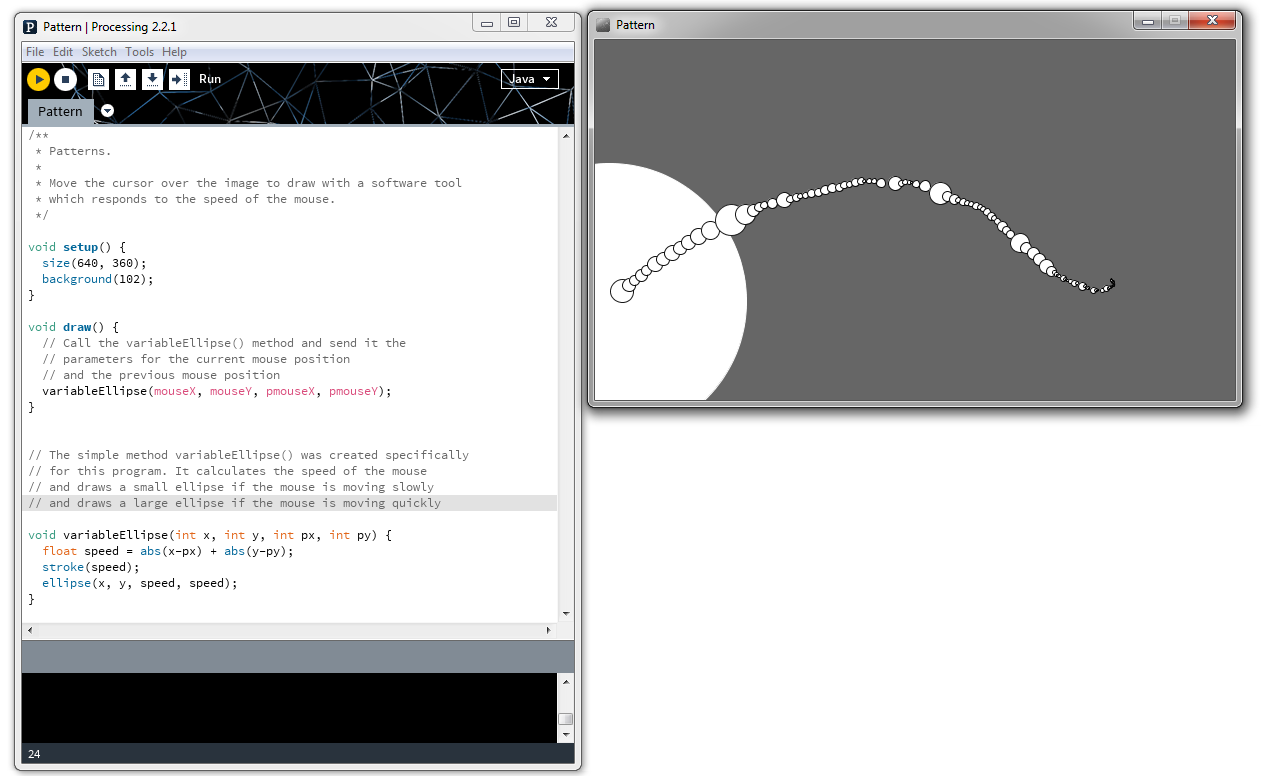
\includegraphics[width=1.0\textwidth]{img/proc_dev_env}
	    \caption{On the left: The \ac{pde} displaying an example \emph{sketch} while it is being run. On the right: The drawing window to which the \emph{sketch's} instructions are applied.}
	  \label{fig:proc:dev:env}
	\end{figure} 

	%\subsection{Processing vs Programming for Everyone}
	%This is a comparison with Java. It can be seen as a limitation.
	Looking at the code in \ref{lst:simple:processing} also reveals the language's resemblance with Java. The same code fragment in Java declares two methods named ``setup'' and ``draw'' that return nothing; both methods belong to whatever class they happen to be inside of; and both have a list of statements to be executed sequentially when they are invoked. Processing's instructions, functions and sketches map to Java's statements, methods and classes.
	%Classes inside sketches are mapped into inner classes.

	%Describe what the language and the environment lack to improve the programming experience for its users and uses (arts). 
		%Describe how it is just a quick start package for graphics programming in Java. 
		%Describe how the environment not only lacks a debugger but also doesn't give proper error messages when something fails and doesn't provide other ways to follow the program execution.
	%Describe how the environment fails to be a better environment than those used in industry software production (like Eclipse).
		%Describe how its users are required to look for documentation when programming.
		%Describe how little feedback the environment provides. E.g. he has to run the sketch to see if it compiles and runs as he expects. This blocks creation by reaction.
		%Describe how trying to hide Java doesn't make it a better language for learning or producing art. For doing more advanced things, Processing still requires the programmer to know Java; why not learn Java straight away? Processing tries to hide Java's metaphors, its objects; bad idea. (Scala does a better job, I suppose)

\subsection{Impromptu\cite{sorensen2005impromptu}\cite{sorensen2010programming}}
	Impromptu is a programming environment developed to explore manipulation of musical structure in live performance; an \ac{ide} for musicians and sound artists.

	%What is live-performance?
	In the case of Impromptu, live performance takes place as live programming the algorithms that produce the sounds of the music.

	%What does it provide to support live-performance?
	To produce live programming Impromptu brings together four components: an audio synthesizer, a real-time scheduling engine, a Scheme interpreter and an \ac{ide}. The first three components make up the runtime environment while the last provides an interface to it. 

	%Describe live programming experience of impromptu.
	The usage of Impromptu revolves around using its \ac{ide} to send code to the Scheme interpreter. The code can schedule audio to be played later, schedule functions to run later, define or redefine functions and ``variables''. 
	One can use Impromptu to incrementally build an algorithm that produces music. He writes small parts of the algorithm, sends them to the interpreter and then uses those parts to build bigger parts. If not satisfied with a part, he can change its code and send it again to the interpreter.

	%Describe it as a creative tool. As a try of bringing live coding back to the stage (it states that it happened during late 80s and early 90s). It states that live coding performances are extensions to what is called laptop performances.
	%Describe it as being a tool for people interested in making music.  probably have experience with synthesizer software but little programming experience.
	%Maybe include link to live performance video.

\subsection{DesignScript\cite{aish2012designscript}}
	%TODO collections can be used everywhere one thing can be used
	%TODO handling collections (replication guides, etc)
	DesignScript is a programming language that was designed to suite the needs of architecture related design and engineering.

	%DesignScript programming paradigms
	DesignScript uses concepts from multiple programming paradigms like object-oriented, functional and associative programming. Entities have properties that can be either data or functions like in object-oriented languages; functions' most important role is to take some input and produce some output without producing side-effects like in functional languages; and dependencies among variables are retained like in associative languages.

	It supports both imperative (following instructions step-by-step) and associative (propagating changes in a dependency graph) control flows. The programmer can choose to have portions of the code following one type of control flow and other portions following the other.

	%DesignScript primitives
	Being a domain-specific language for architecture, DesignScript includes not only primitives to make building 3d models but also operations from the rest of the architecture process such as energy related analysis and architectural elements (like creating or editing \ac{bim} families).
	\emph{It may be better to provide a list of example primitives and operations.}

	Having modeling primitives close to those normally used in architecture software applications and combining several programming paradigms allows the designer to draw from knowledge about architecture modeling while empowering him to express the processes in which those primitives are used.

	%DesignScript editor(s)
	Editing DesignScript programs can be done either by writing or by creating a graph. The graph is a more natural representation of the dependency graph among the variables of the program when the associative paradigm is being used; it can also be viewed as a data-flow graph. The written representation of DesignScript is a sequence of statements that specify the relationship between a variable and other variables; defining functions, using the imperative paradigm and reassigning variables is also possible; features that are less encouraged by a graph.

	DesignScript is used in several environments. These include a textual editor in Autodesk AutoCAD (Figure \ref{fig:ds:autocad}), a dedicated graph editor called DesignScript Studio (Figure \ref{fig:ds:dsstudio}) and later Dynamo (Figure \ref{fig:ds:dynamo}). Both DesignScript Studio and Dynamo use graph based program editing.

	\begin{figure}
	  \centering
	  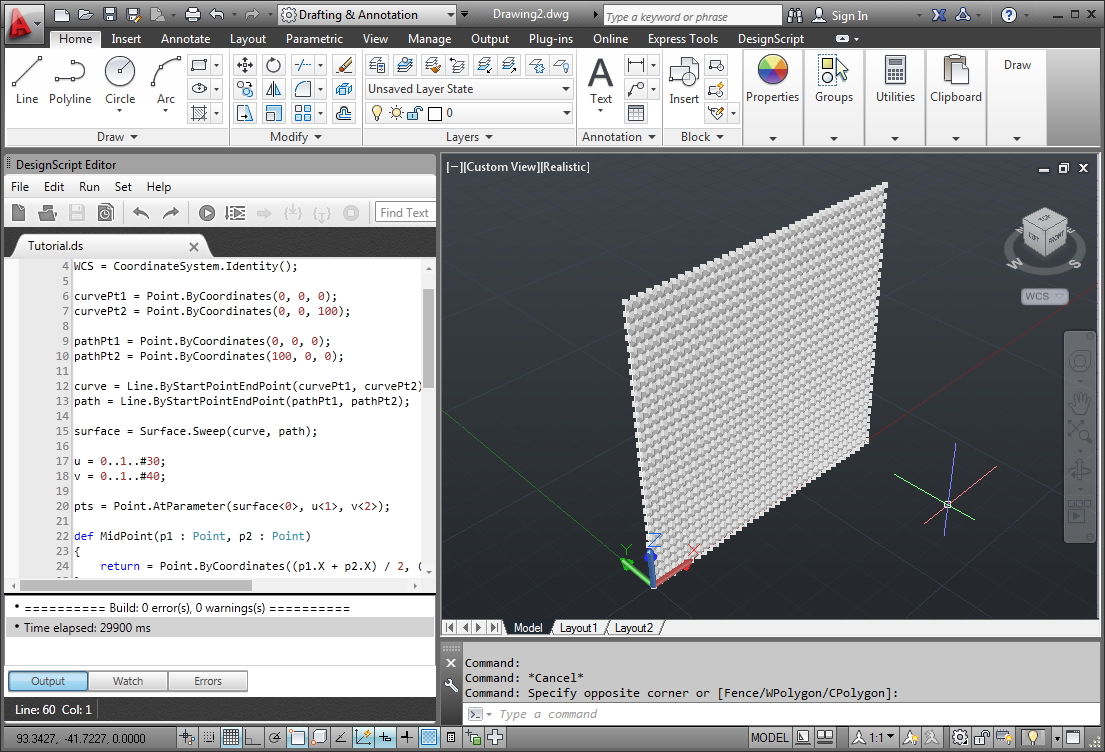
\includegraphics[width=1.0\textwidth]{img/ds_autocad}
	    \caption{A DesignScript program being edited in a special text editor inside AutoCAD. This text editor provides auto-complete and a debugger.}
	  \label{fig:ds:autocad}
	\end{figure} 

	\begin{figure}
	  \centering
	  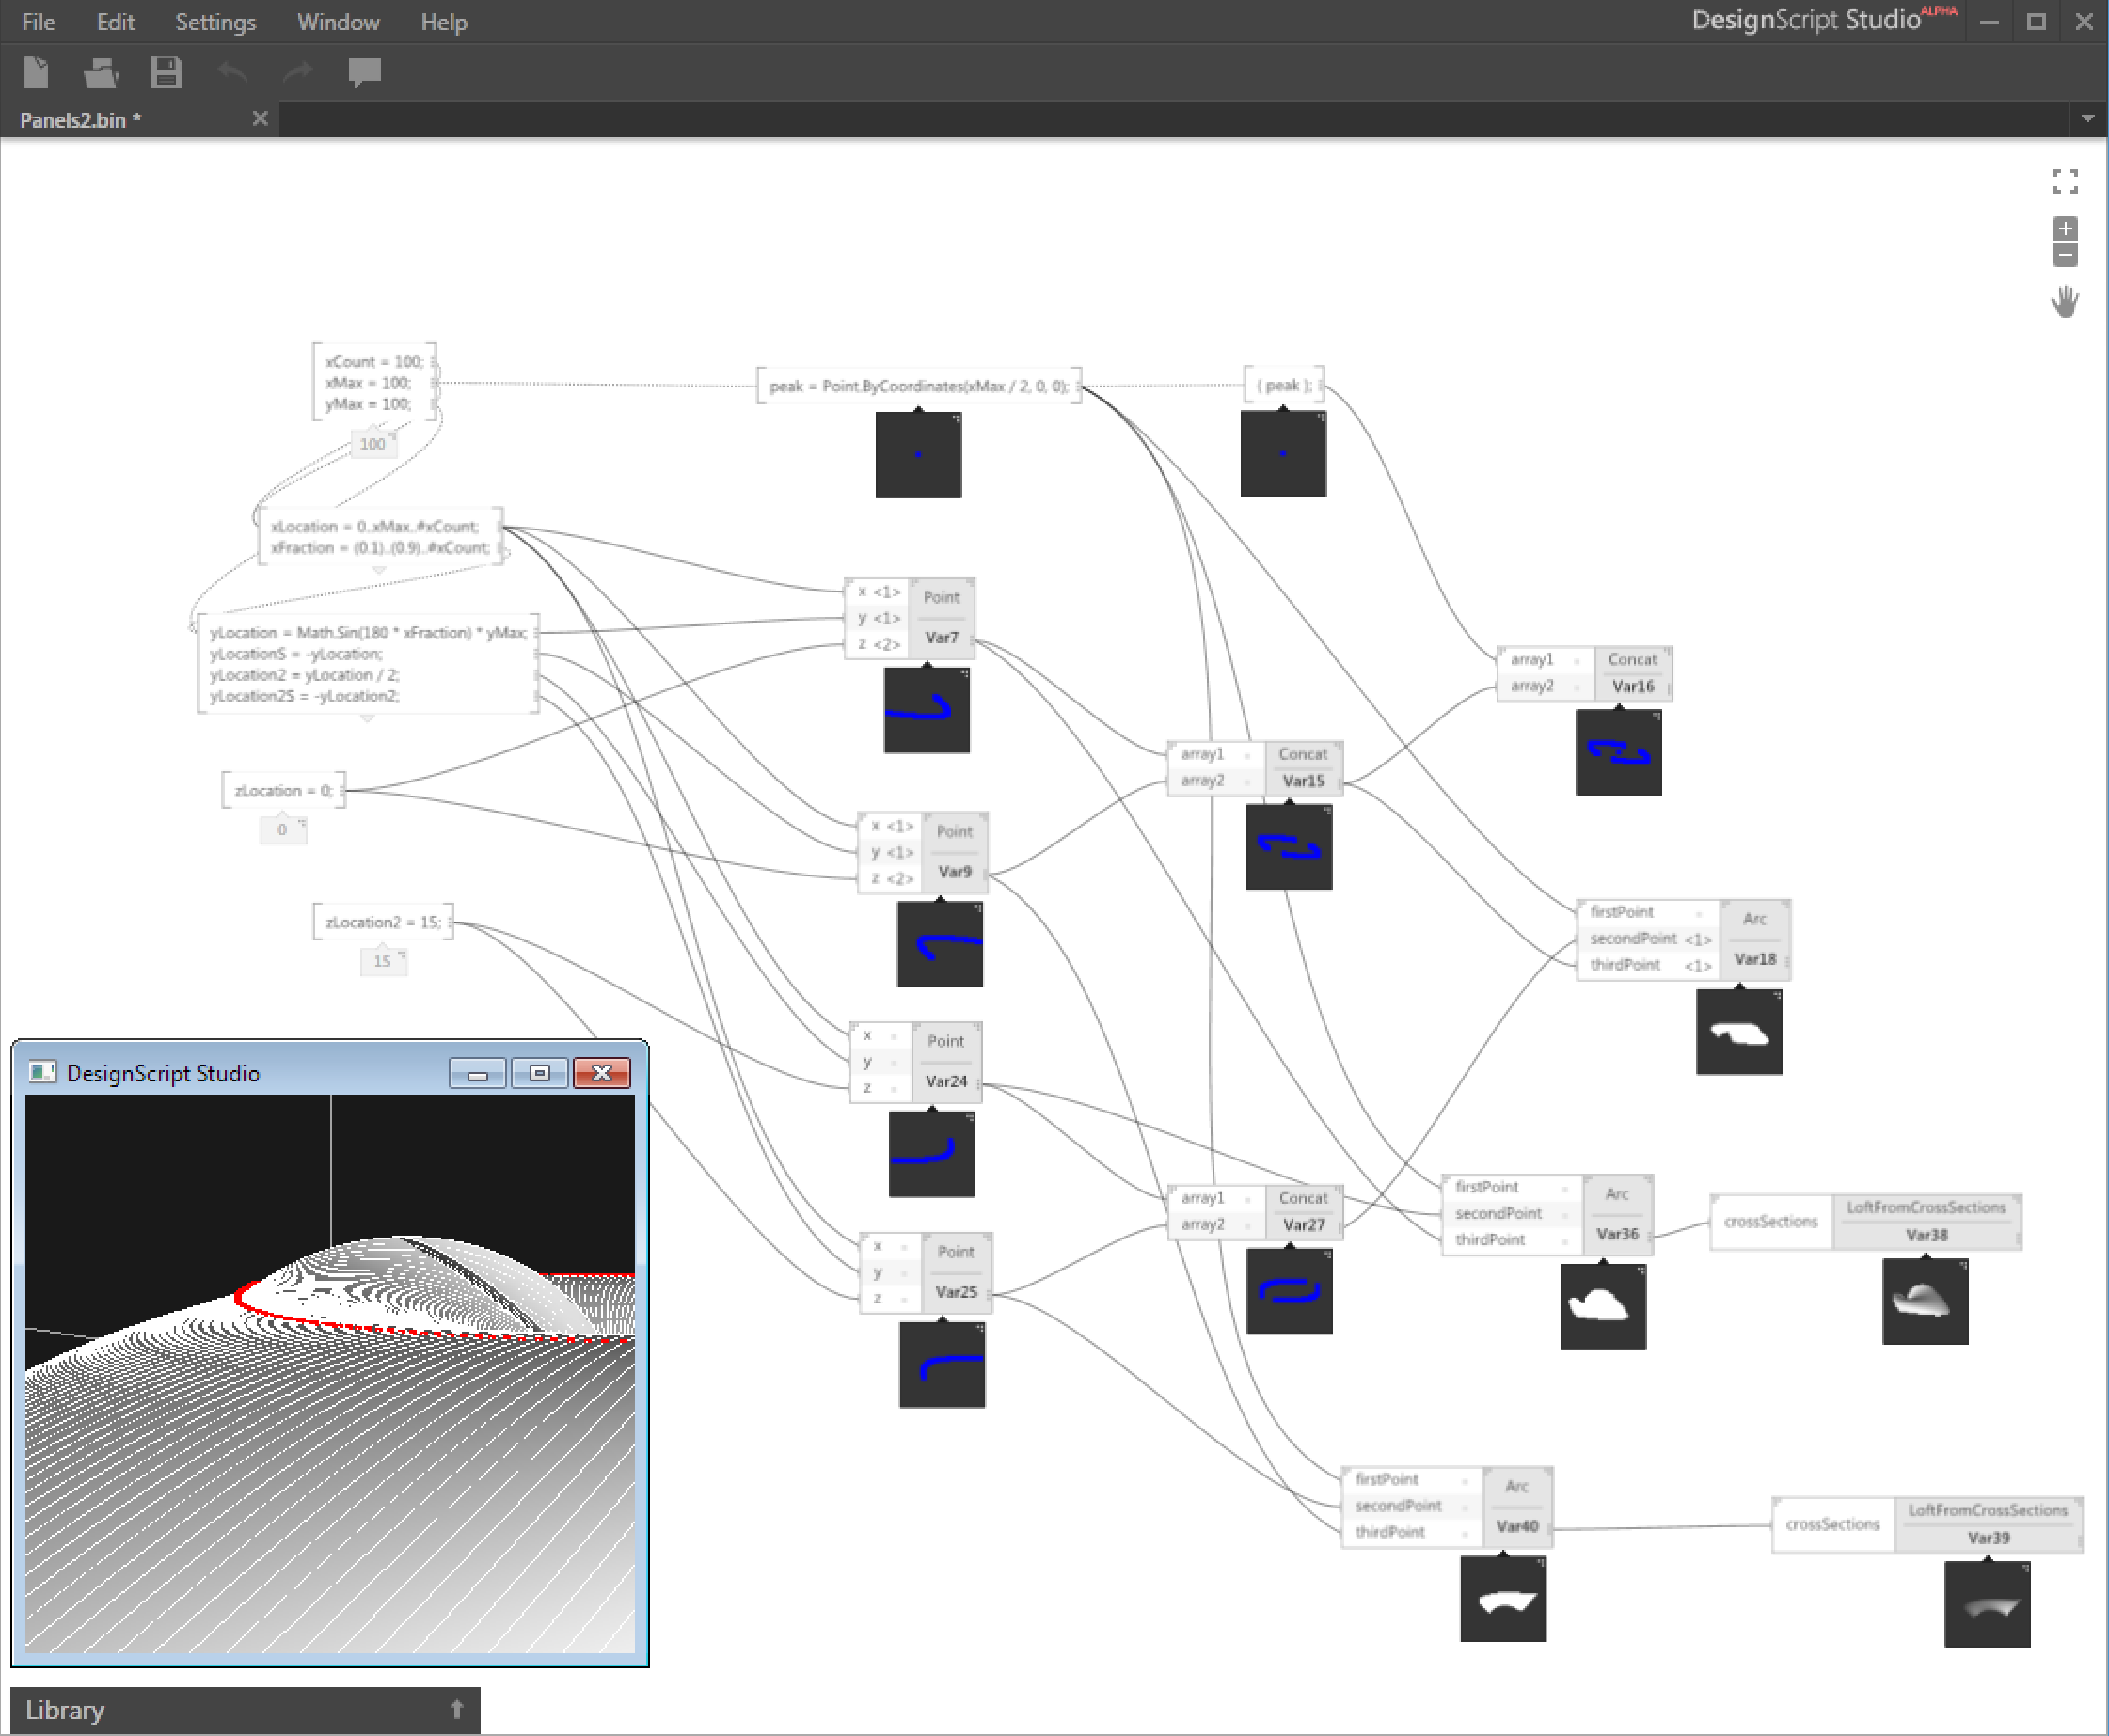
\includegraphics[width=1.0\textwidth]{img/ds_dsstudio}
	    \caption{A DesignScript program as a graph in DesignScript Studio. Each node can display a preview of its results. To the bottom left corner is a preview of the whole program results and a folded library tab. The library tab contains everything that can be used in the program.}
	  \label{fig:ds:dsstudio}
	\end{figure} 

	\begin{figure}
	  \centering
	  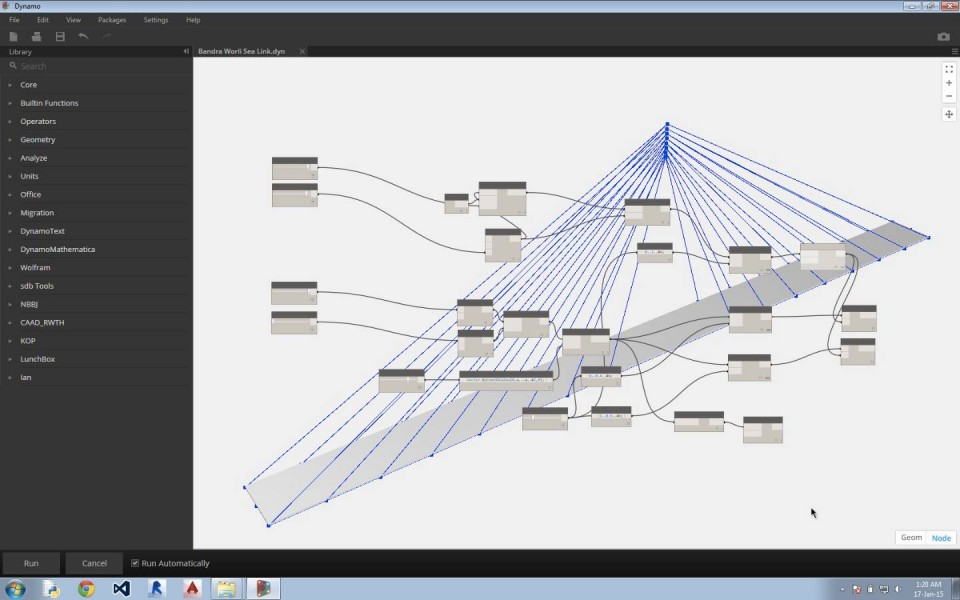
\includegraphics[width=1.0\textwidth]{img/ds_dynamo}
	    \caption{Another DesignScript program as a graph in Dynamo. Like in DesignScript Studio a preview of the result of the program is displayed. A contrast is that there is only one preview ``canvas''; the preview from selected nodes is highlighted.}
	  \label{fig:ds:dynamo}
	\end{figure} 

	Debugging DesignScript programs depends on the environment being used. The textual environment allowed to follow the execution of the program step-by-step while also supporting watches and breakpoints. The graph based environments allow highlighting and listing results of each node. Both the textual and the graph based environments provide a preview of the execution of programs.

	%Editing a DesignScript program is usually done in its dedicated development environment. DesignScript development environment provides auto-complete and debugging capabilities both of which are common features among programming environments.
	
	%DesignScript history
	DesignScript was later used as the scripting language of DynamoBIM, integrated with Autodesk Revit, where programs are edited as data-flow graphs. DesignScript was also integrated into Autodesk AutoCAD. A standalone node-based DesignScript editor was also made, it was called DesignScript Studio.

	%DesignScript problems
	There are some problems that should be pointed out:
	\begin{itemize}
		\item What happens when there are circular dependencies? They can generate infinite loops. It's not clear if it is possible for this to happen.
		\item As with other programming languages being edited using nodes, there is always the risk that programs will become big enough that managing the layout of the graph gets in the way of adding new functionality. 
		\item There is little information on how runtime errors are handled. To my knowledge, the locations where they occur is highlighted and the execution is stopped.
	\end{itemize}


	%It is a multiple paradigm language supporting both imperative and associative programming. At any given point in a DesignSript program, the execution is either being controlled imperatively(following instructions step-by-step) or associatively(propagating changes in a dependency graph). It also uses object-oriented concepts; entities are objects with properties and methods; each object has it's own properties and methods;
	%
	%One way DesignScript tries to succeed is to integrate various ways of modeling into the design process. These various ways of modeling are direct-manipulation mode present in any 3d modeling application, the associative mode present in many visual programming environments and the 

\subsection{IPython\cite{PER-GRA:2007}}
	IPython is a notepad-like environment directed towards providing better, more straightforward scientific computing. \emph{It makes me remember Mathematica's notebooks.} As its name suggests, IPython's main programming language is Python. While Python is its main programming language, other popular programming languages can be used in IPython, particularly those popular in the scientific community like R, Julia. \footnote{More language kernels can be found in IPython's github page: https://github.com/ipython/ipython/wiki/IPython-kernels-for-other-languages}

	IPython was described as a better command line shell.
	When using an IPython notebook -> richer output versus command line interfaces.
	Literate computing

	\begin{figure}
		\centering
		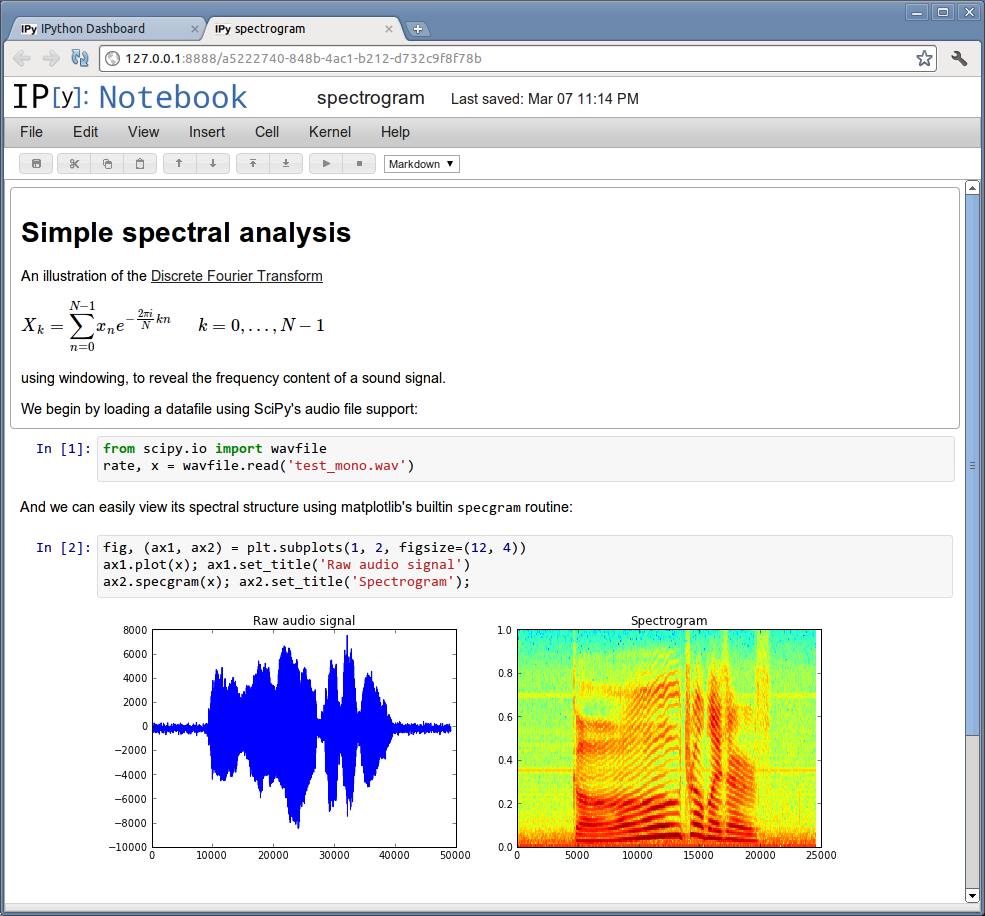
\includegraphics[width=1.0\textwidth]{img/ipython_notebook}
			\caption{An IPython notebook with rich text, mathematical notation, source code and results from executing such code.}
		\label{fig:ipython:notebook}
	\end{figure}

	One trend in its community, one that is supported by IPython notebooks, is to make results in publications more reproducible. Instead of publishing a PDF or making a blog post the authors write whole publications as IPython notebooks which then are shared and thus allow everyone to run their source code. Having access to a working copy of the notebook, one can also experiment with it to better understand it, form own conclusions or find errors.

	Since it aims to be ``A tool for managing the entire lifecycle of a scientific idea''\footnote{Quoting Fernando Perez in his Scipy 2012 Keynote.}, it also provides parallel computation primitives.

	%IPython architecture
	IPython was decomposed into ``execution kernels'', a communication protocol and several front-ends. As each type of component has a defined interface it is possible to implement new specialized components (a new frontend or a new execution kernel) that will integrate with those already implemented.

	%Why is it important? I can't imagine designers using it.
	The style of producing notebooks in IPython is one that mixes programming, writing and exploring. This style is also part of a designer's processes. Like a scientist, the designer also has to do exploration of ideas (design ideas in his case), reach conclusions (crystallized designs) and share his work with others (fellow designers, clients, friends, blog readers). 
	IPython notebooks, more generally notebooks, are natural tools for exploration.
	IPython notebooks don't provide domain specific functionality for architecture.

\subsection{LightTable}
	LightTable is code editor for the Clojure programming language\cite{hickey2008clojure}. It was first written in Clojure and most of its code was later moved to ClojureScript\cite{10.1109/MIC.2011.148}, a subset of Clojure that compiles to Javascript.

	%Disclaimer
	Most of the features described here are only present in LightTable's several experimental versions. The release version's features are not what matters. The ideas behind the experiments are.

	%Why is LightTable relevant?
	%As of now, LightTable doesn't seem to be fulfilling its potential.
	LightTable uses the drafting table as its metaphor\footnote{http://www.chris-granger.com/2012/04/12/light-table---a-new-ide-concept/}. The metaphor comes from looking at the way work is done in other fields of engineering, where engineers spread all materials relevant to their work over large tables, from tools to reference information. 
	Instead of displaying the contents of entire files, LightTable divides the code into meaningful units and displays them as small editors spread over the table's surface. In one of its experimental versions, LightTable also supported displaying running programs in the table. Figure \ref{fig:lt:draft:table} shows an example of this metaphor.

	%Eu gosto da metáfora. Mas não consigo vendê-la aos cepticos; precisa de bastante espaço de ecrã. O que não é mau mas eles só pensam no agora.
	%Maybe I'll have to add a phrase or two to clarify that I'm not targeting software development. Although I would love to be able to come up with something like this that worked for them.

	\begin{figure}
	  \centering
	  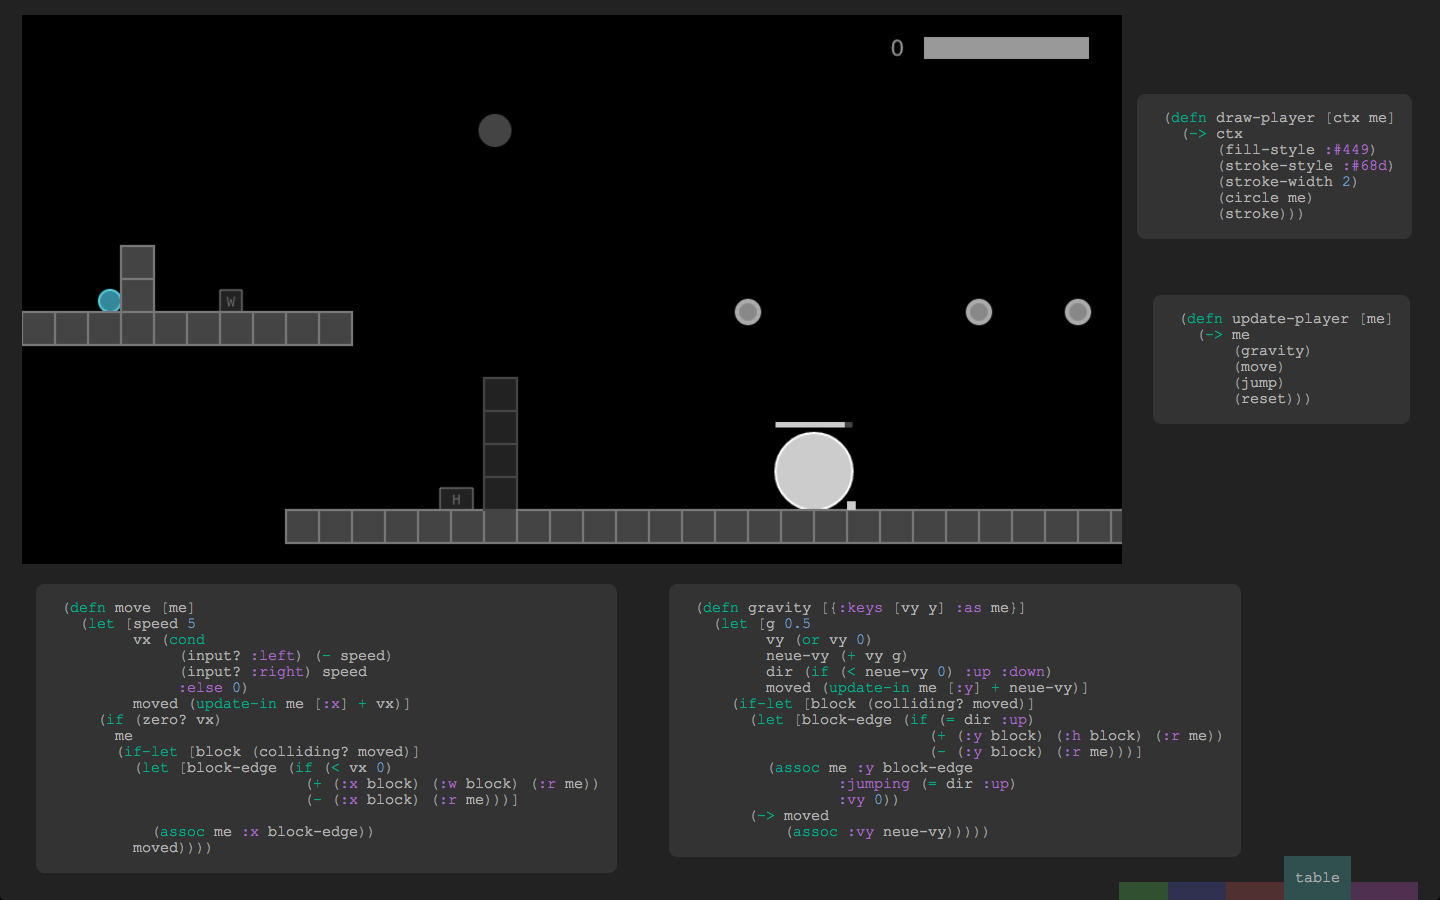
\includegraphics[width=1.0\textwidth]{img/lt_game_example}
	    \caption{A prototype version of LightTable. A game is being run inside it while some of its code is displayed in separate editors.}
	  \label{fig:lt:draft:table}
	\end{figure} 

	%LightTable "function navigation"
	In Clojure functions are defined inside namespaces and all Clojure definitions (functions, variables, macros) are stored in text files. Navigating among definitions and the current namespace structure shouldn't get in the way of editing code. To make editing easier, LightTable provides a \emph{namespace browser} that eases finding functions and a \emph{code document} where functions can be added for editing without moving them out of their namespace or displaying entire files where they are defined. Figure \ref{fig:lt:clojure:table} shows an experiment where these two are used.

	\begin{figure}
	  \centering
	  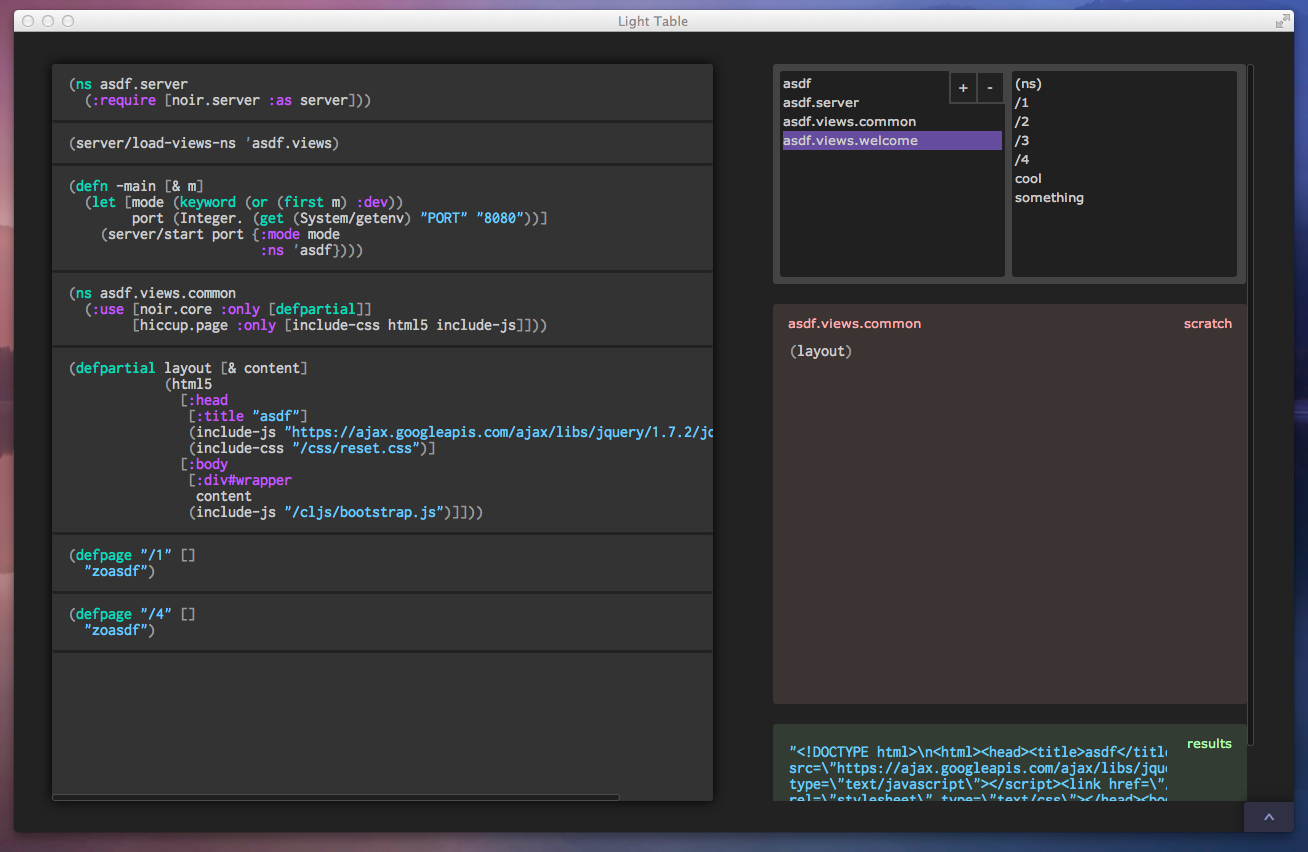
\includegraphics[width=1.0\textwidth]{img/lt_clojure_table}
	    \caption{An experiment showing a \emph{code document} on the left and a \emph{namespace browser} on the top right.}
	  \label{fig:lt:clojure:table}
	\end{figure} 

	%LightTable "variable substitution"
	One interesting functionality of LightTable is its ability to show data flow in a function call. Since the main purpose of a function is to transform its input data into its output data, it helps to see what happens to the data on each step of the function. To achieve this LightTable overlays variable values and return values, respectively, on each variable occurrence and expression of the function. Figure \ref{fig:lt:val:overlay} shows an example of such functionality. This functionality is part of LightTable's \emph{instarepl}.

	\begin{figure}
		\centering
		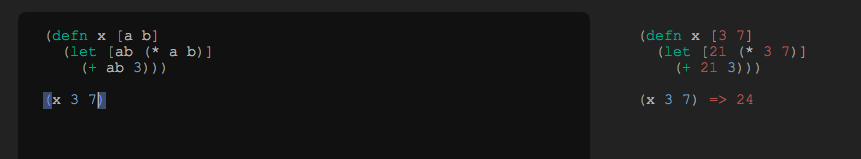
\includegraphics[width=1.0\textwidth]{img/lt_val_overlay}
			\caption{An example of LightTable's value overlaying. The occurrences of the variables \emph{a}, \emph{b} and \emph{ab} were replaced with their values while evaluating the expression \emph{(x 3 7)}; the result of this expression is also overlaid.}
		\label{fig:lt:val:overlay}
	\end{figure}

	LightTable's interface was built on top of NodeWebkit\textsuperscript{citation needed}.

	The main design pattern used in LightTable is the \ac{bot} pattern. As described by one of its developers\footnote{http://www.chris-granger.com/2013/01/24/the-ide-as-data/}, LightTable can be described as a set of \emph{Objects}, each having a set of \emph{Behaviors} and being tagged with a set of \emph{Tags}. The \emph{Behaviors} describe how an \emph{Object} reacts when events are raised on it. \emph{Tags} are groups of \emph{Behaviors}. When an event is raised on an \emph{Object} both its \emph{Behaviors} and those from its \emph{Tags} are notified.


\subsection{Code Bubbles, Code Canvas and Debugger Canvas}
	Code Bubbles and Code Canvas approach displaying and editing program code in a different way from the usual text-based code editors. Instead of showing a programming project as a set of tabs (containing code) and a set of windows (containing tools), they show everything using ``bubbles'' on a virtual 2D surface. The surface view can then be panned and zoomed in and out for navigation.

	As the user explores the code base -- following variables, finding declarations -- new bubbles are created containing the code they want to see.

	Bubbles are laid out in the surface so that they aren't on top of each other. The user can drag the bubbles to change the layout to one that better suits his current needs (e.g. to better reflect the structure of the code or call follow).

	Bubbles can contain code, notes written by the user, debugging information (call stack, local variables' values). They can be grouped together and moved like so when necessary.

	After a usage session, the virtual surface can be saved for later resuming the session or for reference.

	Debugger Canvas, a Visual Studio plug-in, was developed by the teams behind Code Bubbles and Code Canvas to test their approach in the industry setting. According to their results, the approach is most suitable for debugging sessions when the code base is big or when the control flow is complex. It also appeared to be best integrated into professional programmer's tools (IDEs) as a new mode rather than a replacement.

	\textbf{Since we are aiming at architects we can ``assume'' that the kind of interface provided by these works is ``of some use''}.

	%Distintion between Code Bubbles and Code Canvas
	Code Bubbles picks up on the observation that programmers working on a task usually limit the amount of code they see to a working set. In Code Bubbles, the programmer builds the working set as he explores the code base; the built working set is represented as a set of bubbles.
	Code Canvas shows an entire software project as a 2D map. The map can reflect the file structure of the project and/or its semantic structure (e.g. namespaces, classes, methods in OOP projects). Several layers can be overlaid on top of the map such as search results or call stack visualization. The map can be filtered according to some criteria while maintaining positions relative to the entire, unfiltered, map.

	%Why are these important for my project?
	They both provide a metaphor where navigation around a programs code is intuitive. Having intuitive navigation enhances exploration; such exploration makes it easier to understand the code and to have new ideas (the parts bucket is on the floor as in Bret Victor's create by reacting).

	%Is the debugging from these of any use to architects?
	The debugging capabilities from these can help architects (or learners) to explore code from others, be it example code, parts of other projects or even code they wrote but have already forgot how it worked.


\subsection{Rosetta}
	Rosetta is a platform for Generative Design. It grew from the desire to give the freedom to designers using the Generative Design to write their programs using the programming language they want and to easily switch where it takes effect.

	Its authors argue that most environments for Generative Design, developed for a specific CAD, don't provide portability of programs developed inside them. They also argue that visual programming languages, based on data-flow graphs, don't provide good abstraction mechanisms; programs on such languages are therefore hard to understand and modify.

	It is also stated that general purpose programming languages, like C, C++, Java and C\#, don't provide domain-specific abstractions from Generative Design and so they are inadequate.

	A survey of the most used GD systems showed that the most popular TPLs for GD, like AutoLisp, RhinoScript, and GDL, are old, provide little domain-specific features and make it difficult to define them. It also showed that VPLs for GD, like Grasshopper and GenerativeComponents, enforce a very restricted programming paradigm and programs scale poorly with size and complexity, making them suitable only for small throwaway prototypes. It also showed that CAD applications, being based on direct user interaction and imposing their own programming environments and languages, lock their users to the application's product family and make it difficult to achieve correctness, performance and portability.

	The design principles followed by Rosetta are:
	\begin{itemize}
		\item portability (program independence from CAD applications) (enabling reuse of programs across different CAD application communities)
		\item parametric elements (don't require designers to manually transform parametric elements into geometric shapes CADs understand)
		\item functional operations (operations don't consume their arguments) (don't leak CAD implementation details into Generative Design languages)
		\item dimension independent operations (uniform, predictable treatment of shapes of different dimensions)
		\item algebra of sets (shapes as point sets in three dimensional sets) (support for operations on sets)
		\item algebraic equivalences (to handle support discrepancies of set operations across CADs and for optimization)
		\item traceability (between the parts of the program and their results)
		\item immediate feedback (to changes made to the program and its input)
	\end{itemize}

	A modern programming environment for Generative Design should:
	\begin{itemize}
		\item be pedagogic
		\item provide domain-specific features
		\item provide multiple Programming Languages
		\item provide multiple CAD applications
	\end{itemize}

	Generative Design needs:
	\begin{itemize}
		\item Portability
		\item Mathematical and geometric strictness
		\item Correlation between programs and models
		\item Multiple paradigms and techniques
		\item Modern and pedagogic system
	\end{itemize}

	It enables this by providing several ``frontend'' programming languages and several ``backends'' which take the results of the program. The programs written in a ``frontend'' language are compiled into an intermediate language which them translates its semantics to the selected ``backend''.

	Some ``frontends'' supported by Rosetta are AutoLisp, Javascript, Racket and Python; some of the supported ``backends'' include Autodesk AutoCAD, Autodesk Revit, Sketchup, Rhinoceros 3D, TikZ and OpenGL.

	Rosetta has been extensively used for teaching programming to architecture students at \ac{ist}. 


\subsection{Javascript and the Web browser}
	%Mainly from Brendan Eich's presentation "Javascript at 17".
	Javascript began as the Visual Basic for web browsers. It was aimed at web designers that wanted their pages pages to change dynamically. It was inspired by the programming languages Scheme and Self.

	Its first version was developed over ten days during May 1995. It was a quick prototype. 
	During its life it has been loved and hated; it was developed very close to HTML. Like HTML, it had to keep backwards compatibility which made it difficult to fix the bad choices from its first version.

	Having begun in a competitive setting (the web browser), where multiple vendors have their own implementation and coverage of the language, Javascript's standardization has had difficult periods where not all vendors offered the same compliance to the standards (even adding different features).

	Due to the large demands from its users Javascript and web browsers have evolved into a ``reliable platform''. 

	As time passed, Javascript/web standards compliance has been greatly improved. Javascript's performance has also reached the level of native machine code as a lot of effort was put into making Javascript engines fast.

	Currently, Javascript's (or ECMAscript as it is officially called) standards aim to make it a better compiler target language and also for writing applications and libraries. The rationale behind this being the ubiquity that Javascript currently has; every computer now supports Javascript; turning it into a platform that can run anything is very promising (compared to making a new platform from scratch).

	With the recent focus on becoming a target language for compilers, Javascript is sometimes metaphorically called the x86 (or the assembly) of the web.

	Some examples of languages compiled to Javascript are ClojureScript and CoffeeScript. There are many more languages that compile to Javascript. In fact, even C and C++ can be compiled to Javascript\footnote{e.g. with ecmscripten} (or a subset of it\footnote{like asm.js, that aims to be an Ahead-Of-Time compiler friendly subset of Javascript}) and run with speeds close (2x slower) to those gotten while running native machine code. These speeds are suitable for running complex game engines inside the web browser; in a recent demo (2013) an Unreal Engine 3 level run in the web browser without any plug-ins\footnote{https://blog.mozilla.org/futurereleases/2013/05/02/epic-citadel-demo-shows-the-power-of-the-web-as-a-platform-for-gaming/}.

\subsection{OpenJSCAD}
	OpenJSCAD is a javascript application (or rather, an application based on web technologies). It aims to provide the same functionality as OpenSCAD but using javascript as a base for its language. Most of OpenSCAD functionality is implemented in OpenJSCAD. Like OpenSCAD, OpenJSCAD focuses on creating 3D models for 3D printing (e.g. they are solid).

	To actually model in OpenJSCAD the user has to write a program in either OpenJSCAD's language or OpenSCAD's language.

	It is also possible to import 3D models from files commonly used for 3D printing like STL and AMF files. Upon import, the file's content is converted to a jscad program that produces the same model. (I don't see the point of doing this.)

	OpenJSCAD provides two user interfaces, one command-line interface and one graphical user interface as a web page. The first can be used for batch processing (running programs) while the second integrates an editor to edit a program and a 3D view for viewing the results of that program.

	OpenJSCAD's language supports two syntaxes, one based on message passing (or method invoking) and one based on calling functions. Both of these syntaxes are already present in javascript. Many operations provided produce a new object and don't change their parameters. This allows us to follow a functional programming approach and since there are fewer side-effects to know about it is easier to understand a program written using them.

	Some functions in OpenJSCAD and their parameters.
	function parameters result 
	Each primitive has a lot of options on how to call it.
	Its possible to round the edges of polyhedral primitives.
	Non-polyhedral primitives are always converted to polyhedral approximations.

\subsection{Modelo.io}
	One tool that is sometimes requested by the 3D modeling community is a platform where 3D models can be shared and where discussions about those models can happen. Online 3D model libraries like SketchUp 3D warehouse address to some extent this request, however not completely. While they allow models to be shared online, the way comments are made does not allow natural comments on the model; it's not possible to point at a feature of the model and comment it.

	Modelo.io is a simple online service (lacking better words) where anyone can share 3D models. After being uploaded, the author can share them with anyone. The model's page has a WebGL view where it is presented and where its visitors can leave comments as tags attached to points in the 3d model.

	Although Modelo.io can give designers some ways to collaborate it still just allows the collection of feedback on a version of the model. There is no concept of an evolving model, the author has to upload versions of the same model as separate models. \textbf{Apparently there is a notion of versions https://vimeo.com/83648473 but is not what I expected.}

\subsection{More work on CAD done in the web}


\subsection{Wrapping Up}
	%Summarize the parts of the related work that were major influences of the proposed architecture.

%----------------------------------------------------
%NAVarchitecture
\section{Architecture (2/3pgs)}

\subsection{Proof-of-concept Prototype}
	A small prototype has been assembled to test the concept of a Generative Design environment in the browser.

	Like shown in figure \ref{fig:proto:3d:p:editor}, this prototype consists in a web page with a text editor and a 3D view.

	\begin{figure}
	  \centering
	  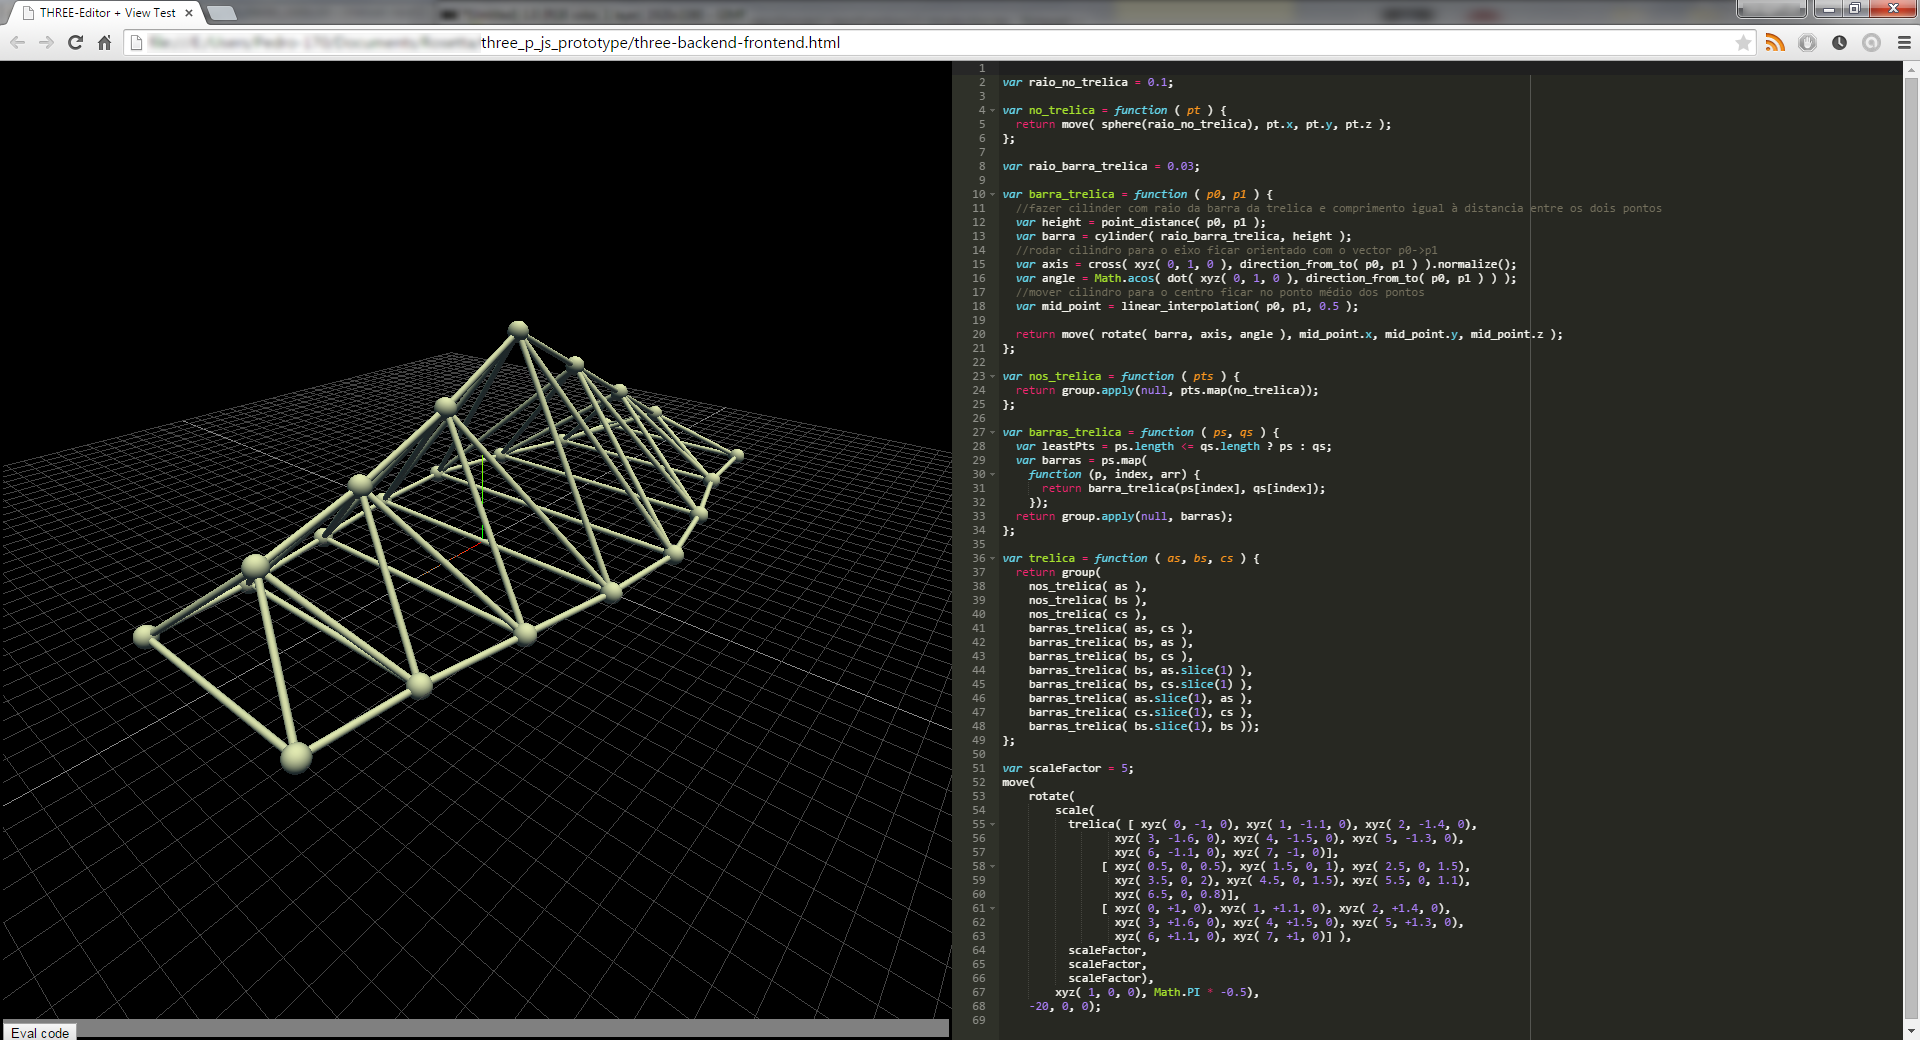
\includegraphics[width=1.0\textwidth]{img/proto_3d_p_editor}
	    \caption{The proof-of-concept prototype generating a truss. The right half contains the program used to generate the truss and the left half contains an interactive view of generated truss.}
	  \label{fig:proto:3d:p:editor}
	\end{figure} 

	The results of running the program inside the text editor are displayed through the 3D view. When the program's text changes, it is rerun to reflect the changes in the 3D view. This enables the prototype to provide immediate feedback to changes as long as they introduce visual changes to the result.

	The user can interact with the 3D view as if it contained a turntable.

	The programming language that is run by the prototype is Javascript with several functions added to produce 3D primitives (such as cubes or cylinders) and to manipulate those primitives (such as moving or grouping).

	The prototype is accompanied with example programs which were used to demonstrate it to a small group of potential users.

	The example programs try to emphasize functional programming techniques like using higher-order functions and minimal use of side-effects.

	The overall feedback from the potential users was positive (they wanted to see it on a real application).

	The prototype is implemented using HTML, Javascript, CSS and two Javascript libraries; the first, Ace\footnote{http://ace.c9.io/}, provides the text editor and the second, THREE.js\footnote{http://threejs.org/}, provides a high-level interface with WebGL rendering.

	With its naive implementation, the use of the prototype has already made clear one problem: always trying to run a program while it is being changed can lead to poor responsiveness or even permanent lockup of the interface. The usual cause being the increasing complexity of the program or the presence of infinite loops in the program. This problem will have to be addressed in order to have a usable interface. Some alternatives to solve the problem could be running the program asynchronously and retrieving the results afterwards or instrumenting the program so it could be run interleaved with interface handling and stopped if necessary.

\subsection{Aspects of the solution}
	One aspect that has to be set is what is the language used to make the programs. Associative vs imperative. With side-effects vs without side-effects.

	Another aspect is the amount of help or documentation or reaction the system has to support the user while he is thinking about and making the program. In an ideal scenario he is capable of either doing both at the same time or being able to switch \emph{modes} quickly without losing context.

	Another aspect is the implementation of primitives of the language like constructive solid geometry, lofts and sweeps. Many others are needed to make the system useful. Being useful is more important than the number of primitives implemented. This leads to other concern, these primitives have to have some correspondence to primitives available in other tools used in architecture.

	For simplicity it is perhaps better to support only 3D modeling primitives as these can show immediate results for this thesis, e.g. energy consumption analysis is a concern in architecture but will not be immediately supported. Other modeling areas will be overlooked either because of the current lack of knowledge of the author and/or because of the added amount of effort to provide them.

	Other aspect is how the system lets users document the programs they made. It is characteristic to forget how some part of the program works and so documentation is needed (or anything that is faster to understand than to interpret the program directly). The system could support having drawings juxtaposed to the program in addition to previews of results like those present in DesignScript Studio, Dynamo and Grasshopper.

	Other aspect is the persistence of programs between usage sessions and in cases the system crashes. In case of persistence between sessions, the user can close the browser or the tab at any moment, it would be useful to keep record of the current program in some way. In case of persistence in case of crashes, if the user program itself crashed the page it should not be executed immediately to allow its retrieval or edition (as it could crash the page again).

	Other aspect is the way programs can be applied to other modeling applications used by architects. Rosetta uses the concept of selecting a backend, a specific interface to a modeling application. After selecting a backend for a modeling application, Rosetta connects to it and results of running the program are passed to the application. The system could connect to Rosetta which would then connect to the application. This approach requires the setup of a communication channel between the browser where the system is running and Rosetta. The system could alternatively use a language that Rosetta already supports. When the user wants to pass the result of the program to the application he only has to select the desired backend and run the program inside Rosetta.

	%It should enumerate the various aspects of concern to be considered while making the solution. It may as well provide some alternatives to some aspects that are already known. These alternatives can refer to products already available.

%----------------------------------------------------
%NAVevaluation
\section{Evaluation (1/2pgs)}

%----------------------------------------------------
%NAVconclusions
\section{Conclusions}

%----------------------------------------------------
%NAVappendix
\newpage
\appendix
\section{Appendix}
\label{sec:attachments}

%----------------------------------------------------
%NAVacronyms
\begin{acronym}
	\acro{ide}[IDE]{integrated development environment}
	\acro{pde}[PDE]{Processing development environment}
	\acro{bot}[BOT]{Behavior-Object-Tag}
	\acro{bim}[BIM]{Building Information Model}
\end{acronym}

% 
% Bibliography
% 
\bibliographystyle{plain} 

% replace example.bib with your .bib
\bibliography{report} 

\end{document}